\chapter{Introduction}
Chapter one provides an introduction of the project group, the assignment provider and MakerSpace HiØ followed by the reasoning behind the thesis.
Afterwards the chapter provides the table of deliveries for the project as well as a section of methods the project group will use for the project including methods for project management, information gathering, testing and evaluation.
Finally a structural description of every chapter in the the report is located at the end of the chapter.

\section{Project group}
The bachelor group consists of the following four IT students:
\begin{itemize}
    \item Andreas Harnes. 
    Computer Science student with interests in networking and programming.
    \item Celina Marie Kristiansen.
    Computer Science student with experience in databases and big data.
    She has previously been deployed at Logiq where she used Databricks to process data.
    \item Magnus Klerck.
    Information systems student with background as a computer electrician where he worked with IT maintenance and hardware repair.
    He also has an interest in cybersecurity.
    \item Morten Offerdal Kvigne.
    Computer Science student with interests in programming and data security.
\end{itemize}
Celina M. Kristiansen, Magnus Klerck and Morten Offerdal Kvigne have previously been working on projects together.
The three had effective collaborations in their former projects which is reflected in the results they produced.
Due to the effective collaboration the three of them decided to form this bachelor group.

Magnus and Morten had both previously worked with Andreas Harnes and they both believed him to be knowledgeable and as such he was brought in.

\section{Assignment provider}
Østfold University College is a university college located in the county Østfold in Norway. Østfold University College has 6485 students across all the different faculties \cite{total_stundets_at_Hiof}. Østfold University College has two campuses which are located in Fredrikstad and Halden. The different faculties are spread across the two campuses. Campus Fredrikstad is the location for the Faculty of Engineering, the Faculty of Health and Social Studies, and the Norwegian Theatre Academy while Campus Halden is the location for the Faculty of Computer Sciences, the Faculty of Education and the Faculty of Business, Social Sciences and Foreign Languages \cite{Hiof_fakta}. 

MakerSpace is a workspace at Østfold University College at Campus Halden. 
The workspace acts as a playground for students and employees who like to use technology to create something \cite{what-is-makerspace}.
MakerSpace is operated by Michael Andersen Lundsveen and 4 student assistants but all students and employees at Østfold University College have access to the facility 24 hours, 7 days a week
\cite{what-is-makerspace}.
Østfold University College describes the drive behind MakerSpace as:

\begin{displayquote}
The purpose of MakerSpace is to offer students a physical space and an engaging environment with the aim to learn something new by encouraging curiosity and eagerness \cite{what-is-makerspace}.
\end{displayquote}
In addition MakerSpace also acts as an area for lectures, courses and experiments.
They also hold basic programming courses for children during the summer.

MakerSpace is equipped with various equipment related to several fields.
Some of the equipment MakerSpace offers is 3D printers, which can be used to print out different figures and shapes in plastic from a 3D model. Soldering irons for making circuits and soldering components, computers with VR headsets, lego robots and remote controlled drones as shown in figure \ref{fig:makerspace}. MakerSpace also has different tools like screwdrivers, workbenches, pliers, RJ45 crimpers to mention some.

Lastly MakerSpace allows students and employees at Østfold University College to borrow equipment.
Students and employees have to note down their name, their contact information and the item(s) they are lending in a book used to keep track of all borrowed equipment whenever they are borrowing equipment.

MakerSpace responsible Michael Andersen Lundsveen is the assignment provider for the project. 
Michael is the leader and principal engineer for MakerSpace Halden.
He oversees day to day operations and he ensures all equipment is in good condition.
Additionally he is responsible for the repairing or the purchase of new equipment should equipment be damaged or destroyed.
Michael also arranges courses for the MakerSpace employees allowing them to learn how to utilize new equipment, he arranges summer workshops for children during the summer vacations and he sponsors certain arrangements and events at Halden University College.

\begin{figure}
    \centering
    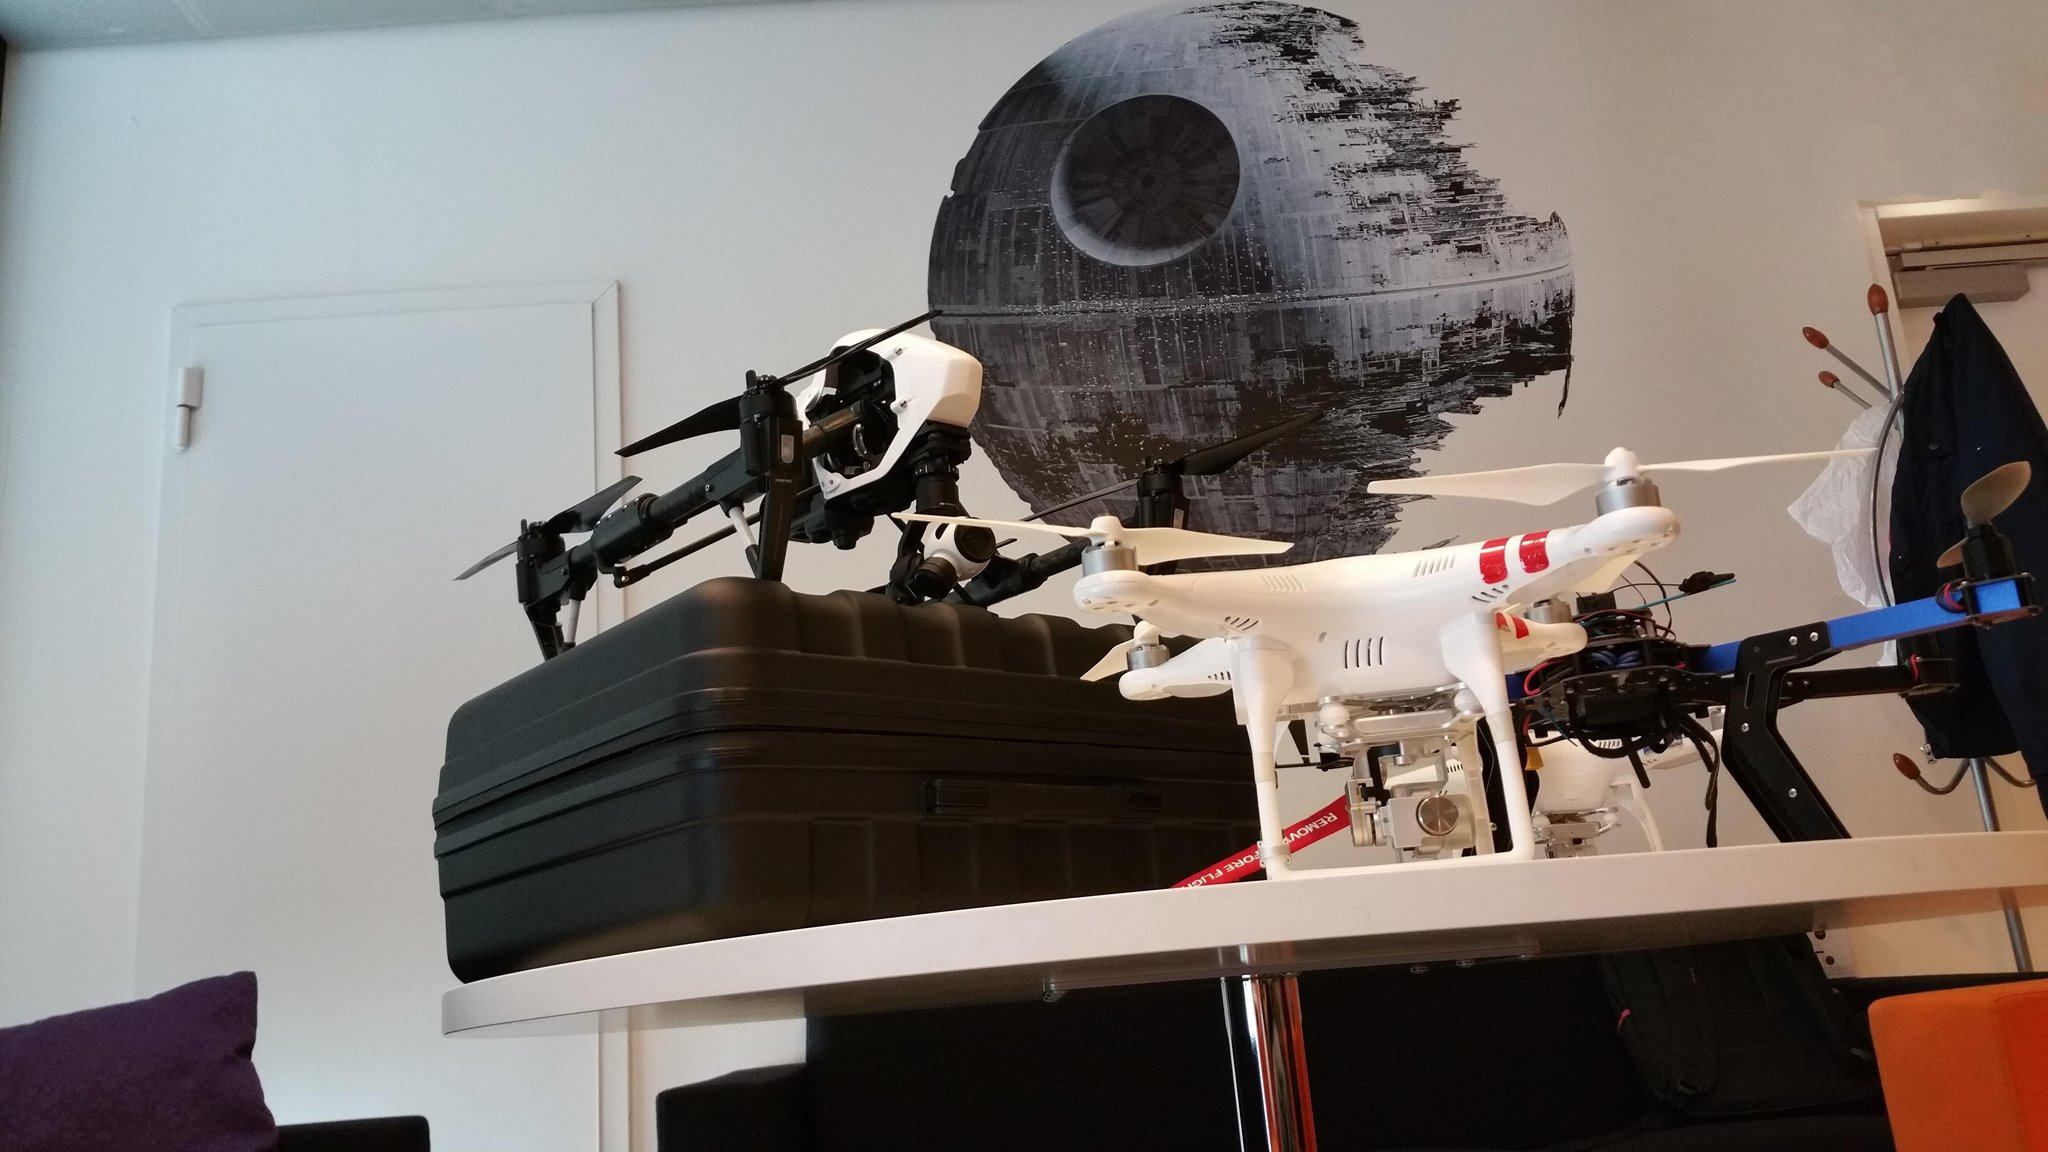
\includegraphics[width=115mm,scale=1]{figures/makerspace.png}
    \caption{Remote controlled drone}
    \label{fig:makerspace}
\end{figure}

\section{The mission}
The background for the project is that MakerSpace currently does not have an overview of what equipment they have, or if the equipment is available and where the equipment is stored.
This is problematic for the employees at MakerSpace as they have no way of knowing whether the equipment is missing or if the equipment is damaged.
Even if an employee is made aware of missing or damaged equipment the employee currently has no way of notifying the other employees and as such the employee will have to manually contact the other employees in order to notify them which is cumbersome.

This is also problematic for the users of MakerSpace.
The users have to search through MakerSpace in its entirety in order to find a given piece of equipment.
They have no way of knowing whether the piece of equipment is damaged until they find it.
They also have no way of knowing whether MakerSpace has the piece of equipment or if another user is currently borrowing it.

Lastly the book used when borrowing equipment also proves problematic.
Anyone can inspect the contents of the book and as such the book does not respect the privacy of the users.
This is concerning should the book be stolen, because all the names and contact information of the users will be astray.
Finally the book is not protected in the event of a fire and all information would be lost.

In order to solve the issues outlined above the group intends to develop two modules.
The employees and users will interact with the modules using web pages.
The following two modules are intended to be developed:
\begin{itemize}
    \item An inventory module allowing employees and users to view the equipment MakerSpace offers, the equipment's condition, where the equipment is stored and weather the equipment is available.
    The module will also allow employees to add, modify and delete equipment from the module.
    \item A lending module allowing employees and users to borrow equipment.
    When returning equipment the module also allows the employee or the user to report any damage that occurred whilst the equipment was being borrowed.
\end{itemize}

The modules will be extendable.
This allows future features to be incorporated into the modules without difficulties for future developers.

%What MakerSpace wants is a system that gives Michael and student assistants access to an overview of all the equipment and tools available in MakerSpace. This system must be modular so that it can be further developed later, and in addition to this a inventory system. They also want a lending module that makes it easier to register the lending of equipment and tools.

%What the group is planning to develop is a modular inventory system and a lending module by adopting technology that is in use today.

%\todo{TODO Alt under flyttes til metode}
%\textbf{Investigation:} The group have talked about some technology they could potentially use. Some of the technology the group have been thinking about is: Vue.js, Node.js and MongoDB. The group will do a investigation for each of those and find out if they fit the project or not. The group will also try and find other technologies that can be more applicable for the project.

%\textbf{Development:} The group will create a website that will offer a lending system of equipment that exists at MakerSpace and also make sure that the system can be further developed later on.

%In the development of the system, the group have made some bullet-points as an overview for the project. These are:
%\begin{enumerate}
%  \item Make the website that will be used for the system and make sure it follow the criteria for universal design.
%  \item Design a structure for the inventory storage.
%  \item Make a module for lending.
%  \item User test the system to find bugs.
%\end{enumerate}

\section{Purposes and delivery}
\subsection{Purposes}
%There are two reasons for the project.
%The first is to provide an overview of the equipment available at MakerSpace to the employees and users of MakerSpace.
%This is beneficial as the employees and users now no longer need to search through MakerSpace in its entirety to see if MakerSpace offers the equipment they seek.

%The second reason is to digitize the lending system MakerSpace currently has in place.
%This is beneficial because it is privacy respecting as only those with the necessary permissions can view the records of equipment currently being borrowed. 
%Additionally should equipment not be returned MakerSpace will know who is responsible.
%Lastly the records of borrowed equipment can be place on a backup - meaning the records of borrowed equipment are not lost in case of theft or in case of a fire.

\textbf{Main goal:} Make an inventory module which provides an overview of the equipment available at MakerSpace.

\textbf{Sub goal:} Make a lending module which digitizes the current lending system used at MakerSpace.

%The purposes with this project is to digitize the current lending system. This will make it easier to not only see what equipment that is available for lending but also what equipment that needs to be order more of. This is divided into a main goal and some sub-goal's.

%\textbf{Main goal:} Digitize current lending system and write the report.

%\textbf{Sub-goal 1:} Make a inventory structure with a lending module

%\textbf{Sub-goal 2:} Make sure that the website (e.g front-end, UI,UX) follow the criteria for universal design.

\subsection{Delivery}

Below are the deliveries the group will deliver during the project.

\begin{tabu} to 1.2\textwidth { | X[l] | X[c] | }
    \hline
    \textbf{Date} & \textbf{Delivery} \\
    \hline
    January 18 ,2019 & Pilot report \\
    \hline
    March 08, 2019 & First version of main document \\
    \hline
    April 23, 2019 & Second version of main document \\
    \hline
    April 26, 2019 & Product \\
    \hline
    May 16, 2019 & Finished version of main document \\
    \hline
    May 27, 2019 & Project poster \\
    \hline
   June 03, 2019 - June 05, 2019 & Presentation of the project \\
    \hline
\end{tabu}
    
\section{Method} \todo{Masse ord som besrkiver lite i 1.5}
\todo{gjør hele kapittelet konkret}
For the project the group will use a set of methods for how the group will conduct research, gather information and how to handle the collected information, what kind of project management method we will use and why it fits the project. The methods used for testing the application and how to most efficiently develop it will also be documented here. 

\subsection{Waterfall} \todo{Legg til figur}
A waterfall model is a sequential project management method which is a linear process of project management\cite{Waterfall_model}. It consists of several discrete phases where no phase begins before the prior phase is complete. Much like a waterfall filling lower level pools, the phases of the waterfall model has six phases where one flow over to the other. The six phases are: Requirements, Design, Implementation, Verification, Deployment and Maintenance\cite{Waterfall_phases}. The reason the group didn't choose waterfall as a project management method is because of the nature of waterfall. The sequential flow of waterfall makes it "impossible" to go back to previous phases. This can be very challenging when going between software development and writing the report. Revisions and changes in both of these can happen at anytime, especially if the scope of the project is changed or planned parts of the projects change during the course of the project.
\begin{figure}
    \centering
    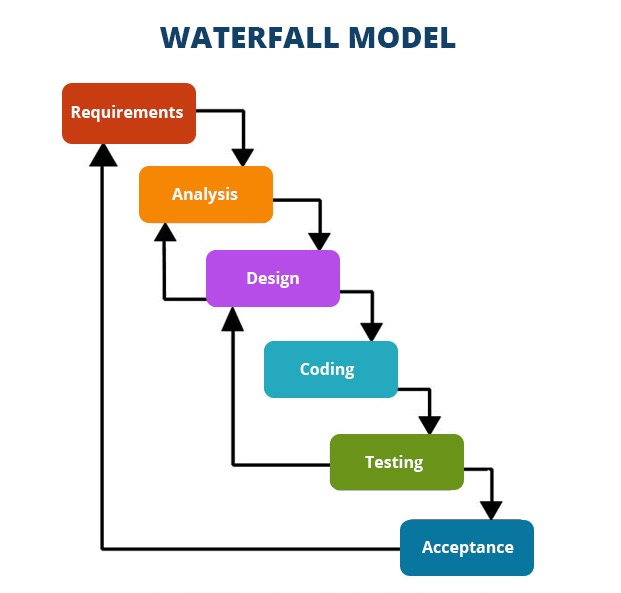
\includegraphics[width=100mm]{figures/waterfallMethods.png}
    \caption{How waterfall works}
    \label{fig:Waterfall_model}
\end{figure}
The right method needs to be used on the correct project, waterfall is most appropriate to use in some situations where:

The requirements are well documented, clear and fixed\cite{SDLC_Waterfall_Model} and the product definition is stable. If the technology is clearly understood and not dynamic, with no ambiguous requirements the Waterfall method could be a good choice. The Waterfall method is also well put in use in situations with ample resources but with the required expertise to support the product and where the project is short. The waterfall model also has several advantages like departmentalization and control where a schedule can be created with deadlines for each phase of the project. As the development moves from one phase to the other and some of the advantages the waterfall model gives are: 
It is simple and easy to understand and use, it is also easy to manage and each phase has specific deliverables and a review process. The Waterfall method is also very suited for smaller projects where the requirements are well understood\cite{Waterfall_Requirement_Advantage}, and the process and results are well documented. 
As with everything the waterfall method has some disadvantages. It doesn't easily allow for changes in the project and when the software reaches the testing stage, going back and making changes to the software can be very challenging if the changes needed to be made haven't been properly documented or thought about in the conceptualization phase\cite{seguetech_waterfall_vs_agile}. Some other disadvantages are: 
There is no working software developed until late in the project and it is not suitable for projects with high risk of changing its scope or other parts of the project\cite{Waterfalls_clear_advantage}. Another disadvantage especially for the project group is that integration for software is done quickly and at the end of the project, which makes it hard to identify any technological or other challenges early\cite{Waterfall_Software_Engineering}. 

So with the waterfall model there are some clear advantages that fits the MakerSpace Management System project.The project is short and the requirements for the project are well documented, clear and fixed. Waterfall works well for smaller projects like MakerSpace Management System and the sequential and step by step phases would give the project more straight forward and easily arranged tasks to complete, which in turn makes the processes and results well documented. And that is very optimal for writing the report for the project. However the waterfall model creates certain difficulties and has some disadvantages that makes waterfall model not the best suited model compared to Agile for this project\cite{seguetech_waterfall_vs_agile}. 

The waterfall model creates a set of challenges. One of these are the development of software isn't started until late in the project. As a lot of the documentation is produced based on the development of software and not only project specifications and analysis of potential technologies i.e. The project has a risk of changing based on revisions on both the software and the report. As progress on both mirrors each other, if changes must be done to the software, some of the documentation might be re-written. This is especially difficult because of the sequential nature of the phases. Where you cant go back to previous phases after they are complete. The scope of the project could also be changed based on time left on the project or challenges with certain components. 

The Agile model is more lenient with making changes on parts of the project and scope. And going back and forth between phases poses less of a problem. Integration of the software in the waterfall model creates a difficult problem as it is integrated late in the project life cycle and gives the group less time to test and identify technological problems and fix them\cite{Waterfall_Model:_What_is_it}. By starting early by implementing and testing the software and making changes to what works and doesn't. It is easier to iron out problems and make sure the release is as smooth as possible. This is best done with Agile, as it works better at handling constant changes in development without causing further problems and risking the entire project. Based on the type of project and possible difficulties, the waterfall model is not the most suitable model for the MakerSpace Management System project.
%\begin{itemize}
    %\item Requirements are very well documented, clear and fixed.
    %\item Product definition is stable.\cite{SDLC_Waterfall_Model}
    %\item Technology is understood and is not dynamic.\cite{SDLC_Waterfall_Model} 
   % \item There are no ambiguous requirements.\cite{SDLC_Waterfall_Model} 
  %  \item Ample resources with required expertise are available to support the product.\cite{SDLC_Waterfall_Model}
 %   \item The project is short.\cite{SDLC_Waterfall_Model}
%\end{itemize}

%\begin{itemize}
 %   \item Simple and easy to understand and use.\cite{SDLC_Waterfall_Model}
  %  \item Easy to manage due to the rigidity of the model. Each phase has specific deliverables and a review process.\cite{SDLC_Waterfall_Model}
   % \item Phases are processed and completed one at the time.\cite{SDLC_Waterfall_Model}
    %\item Works well for smaller projects where requirements are very well understood.\cite{SDLC_Waterfall_Model}
    %\item Clearly defined stages.\cite{SDLC_Waterfall_Model}
%    \item Well understood milestones.\cite{SDLC_Waterfall_Model}
%    \item Easy to arrange tasks.\cite{SDLC_Waterfall_Model}
%   \item The process and results are well documented.\cite{SDLC_Waterfall_Model}
%\end{itemize}

%\begin{itemize}
%    \item No working software is developed until late in the project life cycle.\cite{SDLC_Waterfall_Model}
%    \item High amounts of risk and uncertainty.\cite{SDLC_Waterfall_Model}
%    \item Poor model for long and ongoing projects.\cite{SDLC_Waterfall_Model}
%    \item Not suitable for projects with high risk changing.\cite{SDLC_Waterfall_Model}
%    \item Hard to make room for changing requirements.\cite{SDLC_Waterfall_Model}
%    \item Adjusting the scope of the project can endanger and possibly end the project.
%    \item Integration of software is done very quickly at the end of the project and makes it hard to identify any technological or other challenges early.
%\end{itemize}

\subsection{Agile} 
After looking at the Waterfall model and the Agile model the group has decided to use an agile model for the software development process. After a discussion with the assignment provider about a suitable project management method. The group proposed Agile as the most suitable for the project and the most effective for the type of software development the group would do\cite{Benefits_of_Agile}. The assignment provider agreed to the use of Agile.  
The project is small in scale and is not tightly integrated with any other system. This means the comprehensive documentation a waterfall model requires is not needed before software development can start. Even though Waterfall can be well used for small projects. Additionally this means informal communications between group members work well as the group is co-located.
The agile model does however require a higher presence of the assignment provider as he plays an integral part in which components the group are to prioritize\cite{high_quality_agile}. \todo{Kokludere til slutt}

The assignment provider is involved and accessible throughout the project development.
This allows for incremental development of the requirements set out by the assignment provider which means contract negotiations are not necessary.
Consequently the group can more easily adapt to changes in requirements as the documentation remains largely unaffected by the respective changes.
This is the driving factor behind the agile model:
\begin{displayquote}
Agile is the ability to create and respond to change.
It is a way of dealing with, and ultimately succeeding in, an uncertain and turbulent environment \cite{what-is-agile}.
\end{displayquote}
This is also one of the factors which separates the agile model approach to that of other software development models:

\begin{displayquote}
One thing that separates Agile from other approaches to software development is the focus on the people doing the work and how they work together.
Solutions evolve through collaboration between self-organizing cross-functional teams utilizing the appropriate practices for their context \cite{what-is-agile-software-development}.
\end{displayquote}
With everything taken into consideration the group believes an agile model is more suited for this project than that of a waterfall model.

The group believes the best way to organize the project is using the agile framework Scrum.
Scrum is a framework that is best suited for teams with a size of seven or less \cite{software-engineering-scrum-size} which makes the framework ideal for the group as the group consists of four members.
The assignment provider has set forth the features he would like to see in the system and these features make up the product backlog.
Given the fact that the assignment provider is so involved and accessible it seems fitting that he is involved in deciding which functionality is to be prioritized which Scrum allows him to do as a product owner.
The group believes the flexible approach an agile model used through Scrum provides the best foundation for the successful completion of the project.

%SCRUM (source: https://www.mountaingoatsoftware.com/agile/scrum) will be used as a framework to manage the project and the software development. SCRUM is a derivative of the Agile methodology, but we will use Agile (source:https://www.agilealliance.org) as the methodology when developing software for the project. The Agile method will be used so the group can adjust and adapt to changes in the development as the project goes along. By scaling this to the scope of the group and the project, Agile will fit the development of the project well. 


\subsection{Qualitative and Quantitative methods} When working on the report and documentation for the project it will mainly follow qualitative research methods for gathering information and comparing/analyzing data. Qualitative research method is a scientific method of observation to gather non-numerical data. The aim of a qualitative research project may vary with the disciplinary background, like a mechanical engineer seeking in-depth understanding of a combustion engine for example\cite{Qualitative-Research}. Quantitative methods is when you objectively measure the statistical, mathematical, or numerical analysis of data collected through polls, questionnaires, and surveys, or by manipulating pre-existing statistical data using computational techniques\cite{Quantitative_Methods}.   
 
 Qualitative methods are best for researching many of the why and how questions of something \cite{Qualitative-Research}. Qualitative research is widely used by political science, social work, and education researchers and only produce an explanation for the particular case that is studied. All the qualitative research done for this project will be focused on how we will do something and why that is the best way to do it. Like why did the group choose a certain program over another and how we are going to use said program. The reason for this is that the project does not need any quantitative data for the documentation of the project, two exceptions that might occur is in the testing phase and in a questionnaire that will be sent out. The information gathered from the questionnaire will be about different MakerSpaces in Norway. In the testing phase the project group will ask for a number of students and/or employees to test the developed system and it's ease of use i.g: UI (User Interface), UE (User Experience) and possible bugs. A User Interface is the space where the user (humans) interact with computers (machines)\cite{user-interface}. And the purpose of a User Interface is to make the interaction as effective as possible for a person. Some UI layers could be tactile (touch), visual (sight) and auditory (sound). These layers usually makes up what we know as Graphical User Interface (GUI)\cite{GUI}. The User Experience is about how good, easy and accessible it is to use the competed product. This has everything to do with the customer, and the end user interacting with the product. In the UX the interface, graphics and design is taken into account and planned to be as best as possible\cite{UX}.  
 The data collected from testing could be used to statistically to show that the UI and UX is good for all potential users. No matter how experienced the users are with IT or how many times the users have used the system.

 \subsection{Questionnaire}
 A questionnaire will be made with a selection of different questions aimed at different MakerSpace's in Norway. The questions will be about how they run their MakerSpace and what kind of systems they use, digitally or other to handle their day to day activities. They will also get questions about the equipment they have, what kind of equipment and how they store said equipment. Whether they let people borrow things from them or not and if they have a digital system or any other means to handle equipment being lent out. 
 The questionnaire will be sent out through Google Form to as many Norwegian MakerSpace emails we can find. This is also how the information will be collected. The mail being sent out will kindly ask if they are interested in answering a questionnaire about their MakerSpace. A link will be included to the Google Form. 
 When the answers for the questionnaire comes in. One or more persons from the Bachelor group will go through all of the answers manually. The answers will be compared to each other to map out the differences and similarities between the MakerSpace's. After the answers have been read and compared to each other, they will all be analyzed to see if we can benefit from the answers. By either getting ideas for new functionality, seeing the potential of offering the project groups solution to other MakerSpace's that doesn't currently have a digital inventory solution. Or avoiding issues other MakerSpace's have with their digital inventory solution. The questionnaire will be added as an addendum.          
 
 \subsection{Interview method}
 
 Interviews can be defined as a qualitative research technique. This involves conducting intensive individual interviews with a small number of respondents to explore their perspectives on a particular idea, program or situation.\cite{Interview-Methods} Interviews have three different formats: structured, semi-structured and unstructured.

Unstructured interviews is conducted without any questions prepared before the interview takes place and data is collected in an informal way. This makes unstructured interviews very unreliable from a research standpoint. Answers given during an interview will also vary based on the formulation of the question. Comparing the answers for the questions will then be a challenge due to the different formulation.

Semi-structured interview is like a mix of structured and unstructured interviews. Questions are prepared before an interview and additional questions might be asked during the interview to either clarify, specify or expand on a certain question. 

Structured interviews consists of a set of predetermined questions that all of the interviewees will answer. The questions will be asked in the same order for every interviewee. The data collected from the answers will make data analysis easier because comparing the questions is straightforward. And it is easier to see the contrast between the different answers given.

Interviewing people for the project will have many advantages like the chance to collect detailed information about what other MakerSpaces do, and what kind of systems is in place for loaning out equipment or if they even have a system. By interviewing different MakerSpaces the group has more direct control over the flow of the interview process and has a chance to clarify issues during the interview process. This will make the data collected more accurate and easier to compare to the answers of other MakerSpace branches.

There is however some disadvantages of conducting interviews. One of the disadvantages is the time needed to arrange the interviews at appropriate times for the interviewees and the project group. Each member of the project group would learn most by being present in all the interviews. Being able to see and listen to what other MakerSpaces do would be a better experience than reading a summary or written answers to the interview. Depending on the time needed for other tasks for the project and the interview. The project group will send one person to all the interviews if time is limited.
 
\subsection{Heuristic evaluation}
In a process of developing a system, it can be necessary to do some kind of evaluation and testing\cite{heuristic-evaluation} (see also section below) to get the best end result for a system. One method that the group find suitable for this project is heuristic evaluation. With a heuristic evaluation the group can look into other makerspace system or other systems that have the same similarity and find advantages and disadvantages with how the systems has been designed.

The main point of an heuristic evaluation is to get an expert overview of a system and try to find mistakes that's been made 
under development of the system, this in order to either help improving that system or avoid doing the same mistakes when developing a new system. Alongside trying to find mistakes, you can also with an heuristics evaluation use it to find things that's been done good with the system, and transferring the good ideas to the new system that is under development. 

When conducting an heuristic evaluation, you need some kind of usability principles that is called "heuristics"\cite{heuristic-evaluation}. You can make your own heuristic principles to find out what kind of usability and design you want to look into, and what will be important to look at when you are designing and developing a system. When you are done with the evaluation, you will have a better overview of the system that was been looked at, and what elements that was good and what was bad. By that as previously mentioned you can see what can be improved or what ideas that can be good to have when developing something new. An heuristic evaluation can be a good foundation for developing wireframes but it is important to now that this kind of method doesn't cover everything, so it can be good to combine this method with other tests and methods.\cite{heuristic-evaluation} A good example can be to combine a heuristic evaluation with a usability test method, that can be read about in section below.

If it is impossible the group will try to find other makerspace systems or other systems that have the same similarity, that can be evaluated through an heuristic evaluation, to find out what kind of mistakes or good elements that other systems have, so the group can get some good ideas that they might avoid or implement in the system that is being developed. If the group don't find any other makerspace or other systems that has this kind of a digital system, the group will if possible do an evaluation on a previous bachelor thesis who tried doing the same project as this one. By looking into a previous attempt, the group will see what went wrong and what the other group did well.\cite{heuristic-evaluation}

\subsection{Usability testing}
When the group is done with making a prototype for the system, it can be smart to run a usability test on it \cite{usability-testing}. The main purpose of this kind of testing is to predict the expected performance of an customer using the current system and to detect serious errors before release of the system.\cite{usability-testing}
It will help find difficulties with the prototype and give the group the opportunity to correct the errors before delivery.   

The usability test will need to consist of a test plan (read about the test plan in attachment) that will be followed through the testing \cite{usability-testing}. The test plan consist of a recipe off how to 
to plan and complete the testing and what information that will be collected\cite{usability-testing}. 

The test can be run as many times as desired. In the process of developing a system it can help to run another usability test after fixing the errors from the first test, to detect any new errors that may have appeared after developing some more.

\subsection{Think Aloud method}
Think Aloud is a testing tool that will be used when doing the usability test. \cite{Think_Aloud}
How the tool is supposed to be used is by letting the participant to think aloud when doing the test task he or she has been given. By letting the participant to think aloud will make it easier to discover what the participant really think about the design and the system that has been made. \cite{Think_Aloud}
It will then be easier to know what elements that need to be change to best fit the users needs. 

Some good benefits that the Think Aloud method will offer is: \cite{Think_Aloud} 
\begin{itemize}
  \item \textbf{Cheap.} This method do not need any special equipment to be able to use it. The only thing that will be needed is someone that can sit next to the participant and take notes from what he or she thinks. 
  \item \textbf{Flexible.} It is possible to use this method wherever in a process of developing. Either if it is just a paper prototype or a fully implemented running system. This method can also be used on everyone that is able to tell what they are thinking when doing the test, so that makes it possible to also use this method with users who are visually impaired.
  \item \textbf{Convincing.} When given a direct respond from users and what they think about the design, will be for someone more convincing on what has been tested need a change.
  \item \textbf{Easy to learn.} There are not that many steps to learn, before someone can use this method when doing a usability test. 
\end{itemize}

Although there are many good benefits with the Think Aloud method, it does not mean that there are no downsides. Here is some downsides by using the method: \cite{Think_Aloud} 
\begin{itemize}
  \item \textbf{Unnatural situation.} For most people, they are not used to go around and talk to them self all day. This might makes it hard for the participants to keep up the thinking aloud when doing the test. 
  \item \textbf{Filtered statements.} For some people they want to appear smart when doing the test. This make them to think more detailed before answering, when it is preferred to be given the answer direct. Because of that it is possible to get different result then expected or needed. 
  \item \textbf{Biasing user behavior.} Very often can interruptions change user behavior. In such cases, the behavior doesn't represent the real use, so one cannot base the design on the outcome.
  \item \textbf{Not enough.} Although this Think Aloud tool brings many good benefits, it is not enough to use this tool alone. It is preferable to combine several different tools to get the whole picture of testing.
\end{itemize}

\newpage
\section{Report structure} 
\textbf{Chapter 1, Introduction:}
% Chapter 1.1 contains information about each member of the project group to give more information about who is working on the project. Chapter 1.2 gives into about the assigment provider in this project; Østfold University college. This chapter also contains information about our contact at Østfold University College, Michael Andersen Lundsveen. Chapter 1.3 describes why the project was created, wishes for the project and a scope over the project. Chapter 1.4 is divided  into two sub chapters. The first sub chapter is 1.4.1 Purpose. In 1.4.1 The Goals of the project is described. In chapter 1.4.2 Delivery all the important delivery dates are listed. Chapter 1.5 Method describes the different work methods and approaches that was researched and selected for this project. Chapter 1.6 is the Structure of the report. In this chapter the order and content of every chapter in the report is explained. 
It contains information about the members of the project group and the assignment provider. This chapter also explains why the project was created, wishes for the project and a scope over the project. Here you will also find all the goals and the important delivery dates. Lastly this chapter describes the different research and working methods and approaches that was researched and selected for this project and the structure for the rest of the report. 


\textbf{Chapter 2, Analysis:}
% Chapter 2.1 contains information about different MakerSpace's, what systems they use and how the lab is organized. Chapter 2.2 contains information about all the database technology the project group chose and why it is being used. It also contains information of other database technology that is not being used and why. Chapter 2.3 contains all information about the Frontend technology selection. What the project group chose and why and also other alternatives that were not suitable for the project. Chapter 2.4 contains information about style sheets that are being used, what kind of CSS and why it is being used. Chapter 2.5 contains information about the Backend technology, what kind of technology is being used and why. Chapter 2.6 contains information about how the Frontend and Backend is connected. This includes HTTP and HTTPS, request methods and status codes. Chapter 2.7 contains information about Git and Github, what it is and how it is being used.   
It contains the analysis part of the report. The chapter includes the analysis of the systems used in other Makerspaces and how their equipment is organized, the analysis of different database systems and the groups choices for the project. Description of the analysis for the frontend- and backend architecture and the selection of the technology chosen. And information about other technologies and protocols used in the project.

\textbf{Chapter 3, Design and implementation:}
% Chapter 3.1 contains information about the Frontend and it's design and how it is implemented to look and work the way it does. This includes design choices for both the look and functionality of the web application. Chapter 3.2 Backend contains information about the design and functionality of the Backend for the end-user and what it provides them, with a good look at Endpoints and how it functions. Chapter 3.3 contains information about Frontend and Backend connection and how communication between each other is designed and function. Chapter 3.4 Database contains information about the implementation and design of the database and how it functions.    
The chapter contains information about the design choices and the functionality of the frontend- and the backend architecture are explained. This chapter also contains information and documentation about how the frontend and backend are communicating and the implementation and documentation of the database system.

\textbf{Chapter 4, Testing and Evaluation:}
% Chapter 4.1 contains information about the Heuristic evaluation method to evaluate the project groups web application by comparing it to a similar web application. Chapter 4.2 contains information about the testing of the web application and it's functionality by asking a group of people to use the web application and a detailed test plan.    
It contains information about the different testing methods and interview methods used during testing the application and the result of the testing.

\textbf{Chapter 5, Discussion:}
% Chapter 5.1 contains information about the project groups thoughts on what went well with the project. Chapter 5.2 contains information about the project groups thoughts on what did not go as well as they thought it would and complications during the project. 5.3 contains information about what could have been done differently during the project and what lead the project group to think what they decided to do, could have been done another way. Chapter 5.4 contains information about deviations from the original plan and idea the project group had before and during the project. What was included and what had to be dropped or couldn't be done in time is also part of this chapter. Chapter 5.5 contains information about what the project group learned during the project. What will they remember best and what will they take with them further into work life.
It contains information about the project groups thoughts from the project, complications and what went well in the project. In this chapter you also find information about what the group would have done differently and any deviation from the original plan. In the last part of this chapter there is information about what the group learned during the project.

\textbf{Chapter 6, Conclusion:}
% Chapter 6.1 contains information about the results of the project. What did the project group deliver, does the web application cover the necessary functions and is the developed application usable. Chapter 6.2 contains information about the continuation of the project. What can be built upon the already existing web application and how to hand over access to MakerSpace HiØ. 
It contains information about the results of the project. In this chapter there will be information about the final application, the state of the web application and information about continuation of the project of the application after this project is done.
